%==================================================
%      PREAMBOLO e DICHIARAZIONI INIZIALI
%==================================================
\documentclass[10pt,oneside,a4paper]{article}

\usepackage[latin1]{inputenc} 
\usepackage[italian]{babel}
\usepackage{siunitx} %Inserisce automaticamente i dati con le unit�  di misura correttamente formattate del SI (utilizzo: \SI{0.82}{m^2}, in generale \SI{misura con il punto decimale}{unit�  di misura})
\sisetup{output-decimal-marker = {.}, separate-uncertainty = true, input-uncertainty-signs = \pm, detect-weight=true, detect-family=true} %per usare SI con il punto decimale
\usepackage{listings} %Per citare codice informatico formattandolo correttamente
\usepackage{amsmath}
\usepackage{graphicx}
\usepackage{geometry}
\usepackage{epigraph}
\usepackage{booktabs}	%tabelle migliorate
\usepackage{tablefootnote}	%note a pi� di pagina in tabella
\usepackage{threeparttable} %tabella con note a pi� di tabella
\usepackage{caption}	%descrizione per figure
\captionsetup{tableposition=top,figureposition=bottom,font=small} %setup descrizione
\usepackage{float}
\usepackage{esvect} %vettori
\usepackage{longtable} %tabelle lunghe
\usepackage[dvipsnames]{xcolor}
\definecolor{sepia}{HTML}{80002A}
\usepackage[colorlinks=true, citecolor=black, linkcolor=sepia, urlcolor=black]{hyperref}
\usepackage{mathrsfs}
%\usepackage[utf8]{inputenc}

\usepackage{multicol}
\newenvironment{Figure}
  {\par\medskip\noindent\minipage{\linewidth}}
  {\endminipage\par\medskip}


\newcommand{\var}{\operatorname{var}}
\newcommand{\cov}{\operatorname{cov}}


\usepackage{listings} %Per inserire codice
\lstnewenvironment{codice_c}[1][]
{\lstset{basicstyle=\small\ttfamily, columns=fullflexible,
keywordstyle=\color{red}\bfseries, commentstyle=\color{blue},
language=C, basicstyle=\small,
numbers=left, numberstyle=\tiny,
stepnumber=2, numbersep=5pt, frame=shadowbox,  showstringspaces=false, #1}}{}

\setcounter{section}{-1}

%==================================================
%                  PRIMA PAGINA
%==================================================

\title{\textsc{Studio delle leggi dei Gas}}
\author{\small{G. Galbato Muscio} \and \small{L. Gravina} \and \small{L. Graziotto}}
\date{}

\begin{document}
	\begin{figure}
		\centering
		
\includegraphics[scale=0.5, trim={2.8cm 8.9cm 0 9cm}, clip]{logo.png}
	\end{figure}
	\maketitle
	\begin{center} 
		\fbox{{\fontsize{12pt}{8mm}\textsc{Gruppo B}}} \\
		\vspace{1cm}
		\begin{tabular}{ccc}
			Esperienza di laboratorio && Consegna della relazione \\
			\emph{\small{6 novembre 2017}} &&  \emph{\small{26 novembre 2017}}\\
			\emph{\small{15 novembre 2017}} &&  \\
		\end{tabular} 
		\vspace{0.5cm}
	\end{center}
\hrule
\vspace{0.5cm}
\begin{abstract}
Mediante un sistema pistone-cilindro, collegabile ad una camera di espansione, si studiano le dipendenze di volume, pressione e temperatura di un gas (l'aria) dalle altre variabili di stato, al fine di verificare la validit� delle Leggi di Boyle, Gay-Lussac e Charles. Si realizza quindi un ciclo termico.
\end{abstract}
\newpage
\tableofcontents %Indice
\listoftables %Indice delle tabelle
\listoffigures %Indice dei grafici

\pagebreak
\begin{multicols}{2}

%==================================================
%         SCOPO E DESCRIZIONE DELL'ESPERIENZA
%==================================================
\section{Scopo e descrizione dell'esperienza}
\label{sec:descrizione}
Il modello fisico del \emph{gas ideale}, che � approssimato dai gas reali tanto pi� essi operano a pressioni minori, � descritto dall'equazione universale dei gas,
\begin{equation}
\label{eq:pvnrt}
PV = nRT,
\end{equation}
che lega tra loro, data una quantit� supposta costante di gas, indicata dal numero di moli $n$, durante la trasformazione, le variabili termodinamiche pressione, temperatura e volume, e permette di esprimere l'una in funzione delle altre due; la costante $R$ � detta \emph{costante universale dei gas}, ed ha il valore, qui considerato esatto, $R = \SI{8.31}{J/(mol \cdot K)}$. Tale legge contempla quali casi particolari le tre leggi dei gas di Boyle, Gay-Lussac e Charles, che esprimono una variabile termodinamica in funzione dell'altra, tenuta la terza costante e a prevedendo la stessa quantit� di gas durante tutta la trasformazione.

In questa esperienza si studieranno singolarmente gli andamenti delle variabili termodinamiche tenendo di volta in volta costante una delle tre, realizzando dunque, mediante un cilindro dotato di pistone ed una camera di espansione, trasformazioni \emph{isocore}, \emph{isobare} e \emph{isoterme}.

Si proceder� quindi alla realizzazione di un ciclo termodinamico che, contemplando anche la presenza di una trasformazione \emph{adiabatica}, permetter� di evidenziare come il lavoro compiuto sia diverso da zero lungo un percorso che riporta il sistema allo stato iniziale, e in particolare esso sia pari alla variazione di energia potenziale delle masse utilizzate nel corso del processo.

Per l'analisi dati si utilizzer� un notebook in linguaggio \emph{Python}.


%==================================================
%				APPARATO SPERIMENTALE
%==================================================		
\section{Apparato Sperimentale}
\subsection{Strumenti}
\label{subsec:strumenti}
\begin{itemize}
	\item Pistone in grafite libero di scorrere con attrito trascurabile in un cilindro in pyrex [diametro $\Phi = \SI{32.5 \pm 0.1}{mm}$];
	\item Camera di espansione metallica chiusa da tappo in gomma;
	\item Termometro a mercurio [risoluzione: \SI{0.2}{\degree C}, incertezza: \SI{0.03}{\degree C}];
	\item 2 Calorimetri Dewar;
	\item Tappo per calorimetro;
	\item Bilancia [portata: \SI{8000}{g}, risoluzione: \SI{0.1}{g}, incertezza: \SI{0.03}{g}];
	\item Resistenza elettrica a \SI{30}{V};
	\item Calibro ventesimale [portata: \SI{200}{mm}, incertezza: \SI{0.05}{mm}].
\end{itemize}
\subsection{Sensori}
I seguenti sensori utilizzati sono interfacciati con il software \emph{DataStudio}.
\begin{itemize}
	\item Sensore di posizione angolare, che registra quindi lo spostamento del pistone [risoluzione: \SI{1.e-5}{m}];
	\item Sensore di bassa pressione [risoluzione: \SI{0.01}{kPa}];
	\item Sensore di temperatura [risoluzione: \SI{1.e-5}{\degree C}].
\end{itemize}
%==================================================
%            SEQUENZA OPERAZIONI SPERIMENTALI
%==================================================
\section{Sequenza Operazioni Sperimentali} 

\subsection{Costante di tempo del termometro}
\label{subsec:costante_termometro}


% LEGGE DI BOYLE
\subsection{Verifica della Legge di Boyle}
\label{subsec:Boyle}
\paragraph{Modello fisico ideale}
Un gas a temperatura costante, sottoposto a variazioni di volume, aumenta o diminuisce la pressione esercitata sulle pareti del contenitore mantenendo il prodotto della pressione per il volume costante:
\begin{equation} 
\label{eq:boyle}
PV = \text{cost} \;\;\; \text{\small(\emph{Legge di Boyle})}.
\end{equation}
Da tale equazione, dunque, si prevede un andamento lineare del grafico della pressione in funzione del reciproco del volume. Per piccole variazioni di pressione attorno alla pressione atmosferica $P_0 = \SI{1.01e5}{Pa}$, assumendo costante il numero di moli del gas contenuto nel sistema, si pu� sviluppare in serie l'espressione di $V$:
\begin{equation*}
V = \frac{nRT}{P} \sim \frac{nRT}{P_0}\big[2-\frac{P}{P_0}\big]
\end{equation*}
\begin{equation}
\label{eq:boylelin}
\rightarrow \Delta V = - \frac{V_0}{P_0} \Delta P.
\end{equation}

\paragraph{Sistema reale}
Il sistema termodinamico studiato utilizza come gas l'aria, che per variazioni di pressione piccole se comparate alla pressione atmosferica si comporta sostanzialmente seguendo la legge dei gas. Tuttavia � da tener conto del fatto che vi possano essere consistenti perdite di gas nel cilindro, in quanto il pistone, nella sua corsa, non � ermeticamente aderente al cilindro; ulteriore causa di errore � dovuta alla non precisa determinazione del volume inizialmente occupato dal gas: sono infatti presenti dei tubi per collegare il sistema al sensore di bassa pressione e alla camera di espansione, il cui volume non si � in grado di misurare con la medesima accuratezza. Si stima, tuttavia, che esso sia trascurabile rispetto a quello occupato nel cilindro e nella camera di espansione. 

Il volume occupato dal gas nella camera di espansione viene calcolato a partire dalla misura con un calibro ventesimale, utilizzando i becchi interni e la parte terminale, delle dimensioni della stessa; si ottiene 
\begin{equation*}
\begin{aligned}
\phi = \SI{36.45 \pm 0.05}{mm} \;\; \text{\small (diametro)} \\
\bar{h} = \SI{85.55 \pm 0.05}{mm} \;\; \text{\small (altezza)}.
\end{aligned}
\end{equation*}
Constatandone la forma cilindrica e trascurando il volume occupato dal tappo, piccolo se rapportato a quello complessivo, si ottiene
\begin{equation*}
V_\text{camera} = \Big(\frac{\phi}{2}\Big)^2\pi \bar{h} = \SI{8.93 \pm 0.03 e-5}{m^3},
\end{equation*}
con incertezza calcolata con
\begin{equation}
\label{eq:sigmaV}
\sigma_V^2 = \Big(\frac{\Phi\pi h}{2}\Big)^2\sigma_\Phi^2 + \Big(\frac{\Phi^2\pi}{4}\Big)^2\sigma_h^2.
\end{equation}

La misura del volume iniziale viene effettuata con il pistone e il cilindro in posizione orizzontale e il gas sottoposto alla sola pressione atmosferica; il pistone viene posizionato all'altezza di $h = \SI{0.0650 \pm 0.0003}{m}$, lettura data dalla scala presente sul cilindro e con errore associato dato dall'interpolazione tra le tacche. Noto il diametro $\Phi$ del cilindro, si ottiene il volume del cilindro
\begin{equation*}
V_\text{cilindro} = \SI{5.39 \pm 0.04 e-5}{m^3}
\end{equation*}
dove si � utilizzato
\begin{equation*}
V_\text{cilindro} = h\pi\Big(\frac{\Phi}{2}\Big)^2 
\end{equation*}
e per l'incertezza l'equazione~\ref{eq:sigmaV}. A questo volume va sommato quello precedentemente calcolato per la camera di espansione, ottenendo quindi
\small{
\begin{equation*}
V_0 = V_\text{cilindro} + V_\text{camera} = \SI{1.432 \pm 0.005 e-4}{m^3}.
\end{equation*}
}
\normalsize


La pressione iniziale � invece quella atmosferica, assunta senza incertezza, $P_0 = \SI{1.01e5}{Pa}$.
Da tali valori iniziali, utilizzando la legge dei gas, � possibile fornire una stima del numero di moli presenti nel sistema all'inizio, presa come temperatura quella iniziale del sistema, $T_0 = \SI{25.51 \pm 0.03}{\degree C} = \SI{298.66 \pm 0.03}{K}$, ottenuta come la media con deviazione standard dei primi dieci valori acquisiti dal sensore:
\begin{equation}
\label{eq:nteor}
n_\text{teor} = \frac{P_0V_0}{RT} = \SI{5.83 \pm 0.02 e-3}{mol},
\end{equation}
con errore dato da 
\begin{equation*}
\sigma_n = n\sqrt{\Big(\frac{\sigma_{V_0}}{V_0}\Big)^2 + \Big(\frac{\sigma_{T_0}}{T_0}\Big)^2}.
\end{equation*}

\paragraph{Procedura e presa dati}
L'esperimento � stato condotto nel modo seguente:
\begin{enumerate}
\item Si posiziona il cilindro orizzontalmente, con il pistone all'altezza $h$ discussa precedentemente; si misura volume e pressione iniziale;
\item Si collega il sensore di bassa pressione da un lato all'interfaccia e dall'altro al cilindro; quindi, si pone quale valore di calibrazione la pressione di \SI{0}{kPa};
\item Si collega il sensore di posizione all'interfaccia: esso misura le variazioni di posizione del pistone mediante la rotazione di una puleggia, attorno alla quale scorre un filo solidale con il pistone stesso. Si imposta il software in modo che esso restituisca direttamente il valore della variazione di posizione lineare, traducendo da quella angolare della puleggia;
\item Si esercita fisicamente una pressione lenta e continua sul pistone, al fine di comprimerlo, e si campionano i dati con frequenza di \SI{10}{Hz}.
\item Si ripete il procedimento portando inizialmente il gas ad una temperatura diversa, mediante la camera di espansione, al fine di verificare la validit� della legge anche lungo un'altra isoterma.
\end{enumerate}
La raccolta dati di posizione, in \SI{}{m}, e temperatura, in \SI{}{\degree C}, � stata effettuata con cinque cifre dopo la virgola, mentre quella della pressione, in \SI{}{kPa}, con due cifre decimali. Si assume pertanto come incertezza sul singolo dato l'ultimo digit diviso per $\sqrt{12}$.

\begin{Figure}
\centering
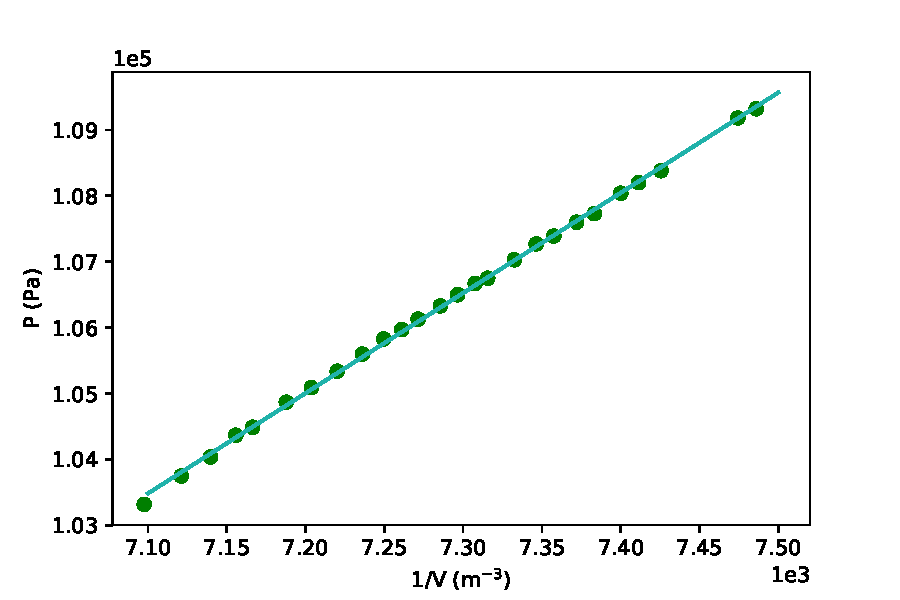
\includegraphics[width=\textwidth]{Pvs1_V.pdf}
\captionof{figure}{Andamento di $P$ in funzione di $1/V$}
\label{fig:Pvs1_V}
\end{Figure}

Alla temperatura media di \SI{298.73 \pm 0.02}{K}, calcolata come media dei valori acquisiti dal sensore per tutta la durata del processo in esame, l'andamento della pressione del gas in funzione del reciproco del volume � riportato in figura~\ref{fig:Pvs1_V}; per ricavare la variazione di volume a partire dalla misura di variazione di posizione $x$ acquisita dal sensore si � utilizzato
\begin{equation*}
\Delta V = x\pi\Big(\frac{\Phi}{2}\Big)^2,
\end{equation*}
e successivamente si � sommato tale valore al valore del volume iniziale $V_0$; allo stesso modo si � operato per la pressione, con $P = P_0 + \Delta P$.

\begin{Figure}
\centering
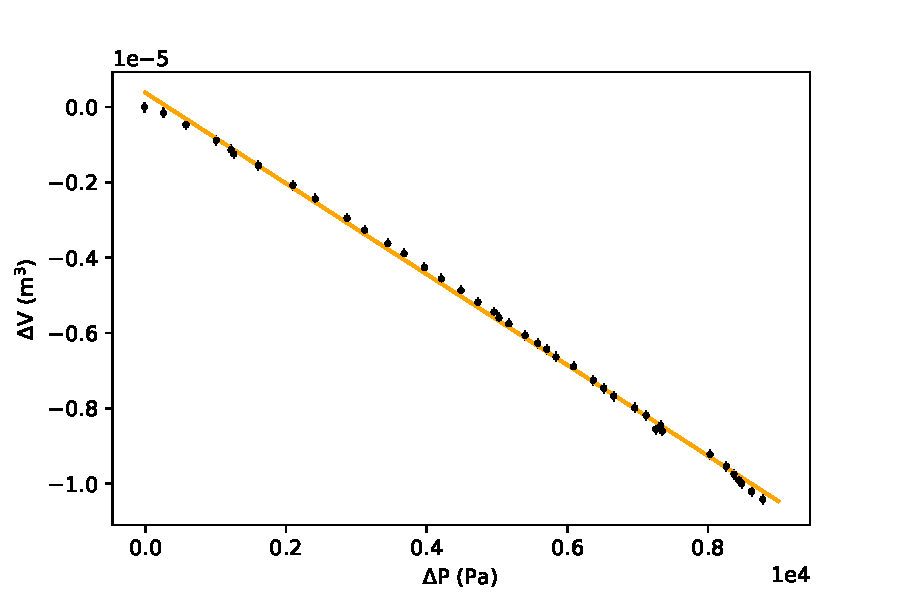
\includegraphics[width=\textwidth]{deltaPdeltaV.pdf}
\captionof{figure}{Andamento di $\Delta V$ in funzione di $\Delta P$}
\label{fig:deltaPdeltaV}
\end{Figure}


Utilizzando invece la linearizzazione della legge data dall'equazione~\ref{eq:boylelin}, si riporta nel grafico di figura~\ref{fig:deltaPdeltaV} l'andamento della variazione di volume in funzione della variazione di pressione. Si procede quindi ad effettuare un fit lineare, ottenendo come valore del coefficiente angolare
\begin{equation*}
m  = \SI{-1.209 \pm 0.004 e-9}{m^3 / Pa};
\end{equation*}
tale valore � accompagnato da incertezza stimata a partire dal chi quadro: quest'ultimo, in prima analisi, risultava non compatibile con il numero di gradi di libert�, dato dal numero di dati meno due, e di molto maggiore, indice del fatto che le incertezze sulla variazione di volume calcolate per ogni singola acquisizione mediante l'equazione~\ref{eq:sigmaV} fossero di molto sottostimate. Si ritiene che questo sia dovuto alla perdita costante di parte del gas nel sistema sottoposto alla riduzione del suo volume, che non � tenuta in considerazione dall'alta accuratezza scelta nell'acquisizione operata dal sensore. Nel grafico rappresentato, di conseguenza, si sono rappresentate con le barre di errore verticale le incertezze sui valori di $\Delta V$ stimate a partire dal chi quadro; al fine di migliorare la leggibilit�, inoltre, si � rappresentato un dato ogni quattro.

Ricordando che $m = - V_0 / P_0$ � possibile stimare dal fit, per mezzo di un metodo indiretto, il numero di moli di gas, supposte idealmente costanti, che hanno preso parte al processo termodinamico; si ha
\begin{equation*}
n_\text{indir} = \frac{P_0^2 \vert m \vert}{R T} = \SI{4.97 \pm 0.02 e-3}{mol},
\end{equation*}
con incertezza data da 
\begin{equation*}
\sigma_n = n\sqrt{\Big(\frac{\sigma_{m}}{m}\Big)^2 + \Big(\frac{\sigma_{T_0}}{T_0}\Big)^2};
\end{equation*}
in questo caso, la temperatura $T$ � ottenuta come media di tutti i valori acquisiti dal sensore nel corso dell'intera durata del processo: $T = \SI{25.58 \pm 0.02}{\degree C} = \SI{298.73 \pm 0.02}{K}$. Tale valore, inoltre, giustifica la assunta isotermia del fenomeno considerato.
Confrontando tale valore con quello teorico calcolato precedentemente (cfr. equazione~\ref{eq:nteor}), si evince che nel corso del processo il numero di moli di gas � diminuito, come era stato previsto dalla considerazione della non perfetta tenuta delle giunture tra i tubi e del pistone stesso nel cilindro.





\subsection{Verifica della Legge di Gay-Lussac}
\label{subsec:Gay-Lussac}

\subsection{Verifica della Legge di Charles}
\label{subsec:Charles}

\subsection{Realizzazione di un ciclo termico}
\label{subsec:ciclo}


%==================================================
%				    CONCLUSIONI
%==================================================
\section{Considerazioni finali}



\end{multicols}




\end{document}
